\begin{appendices}

\begin{figure}[H]
\section*{Dossier médical dans Topaze Maestro}
  \centering
  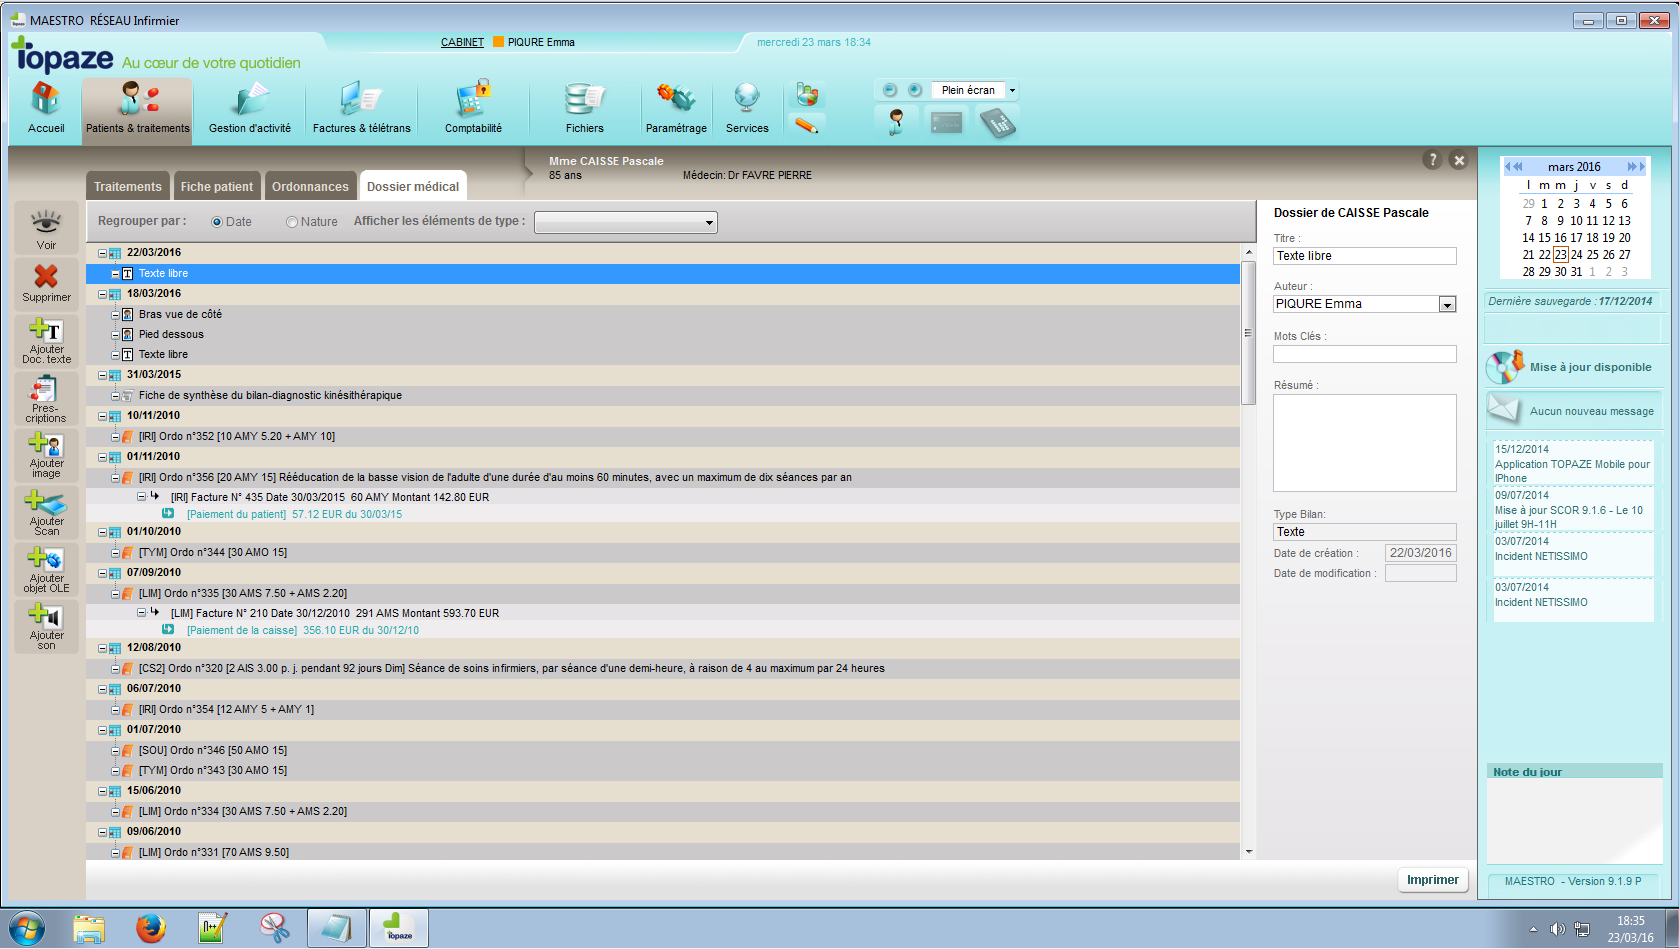
\includegraphics[width=18cm]{./img/medical_data_maestro.PNG}
  \caption{\label{fig:dossier_medical} Dossier médical tel qu'il est présent dans Topaze Maestro.}
\end{figure}

\newpage
\begin{figure}[H]
\section*{L'editeur de texte de Topaze Maestro}
  \centering
  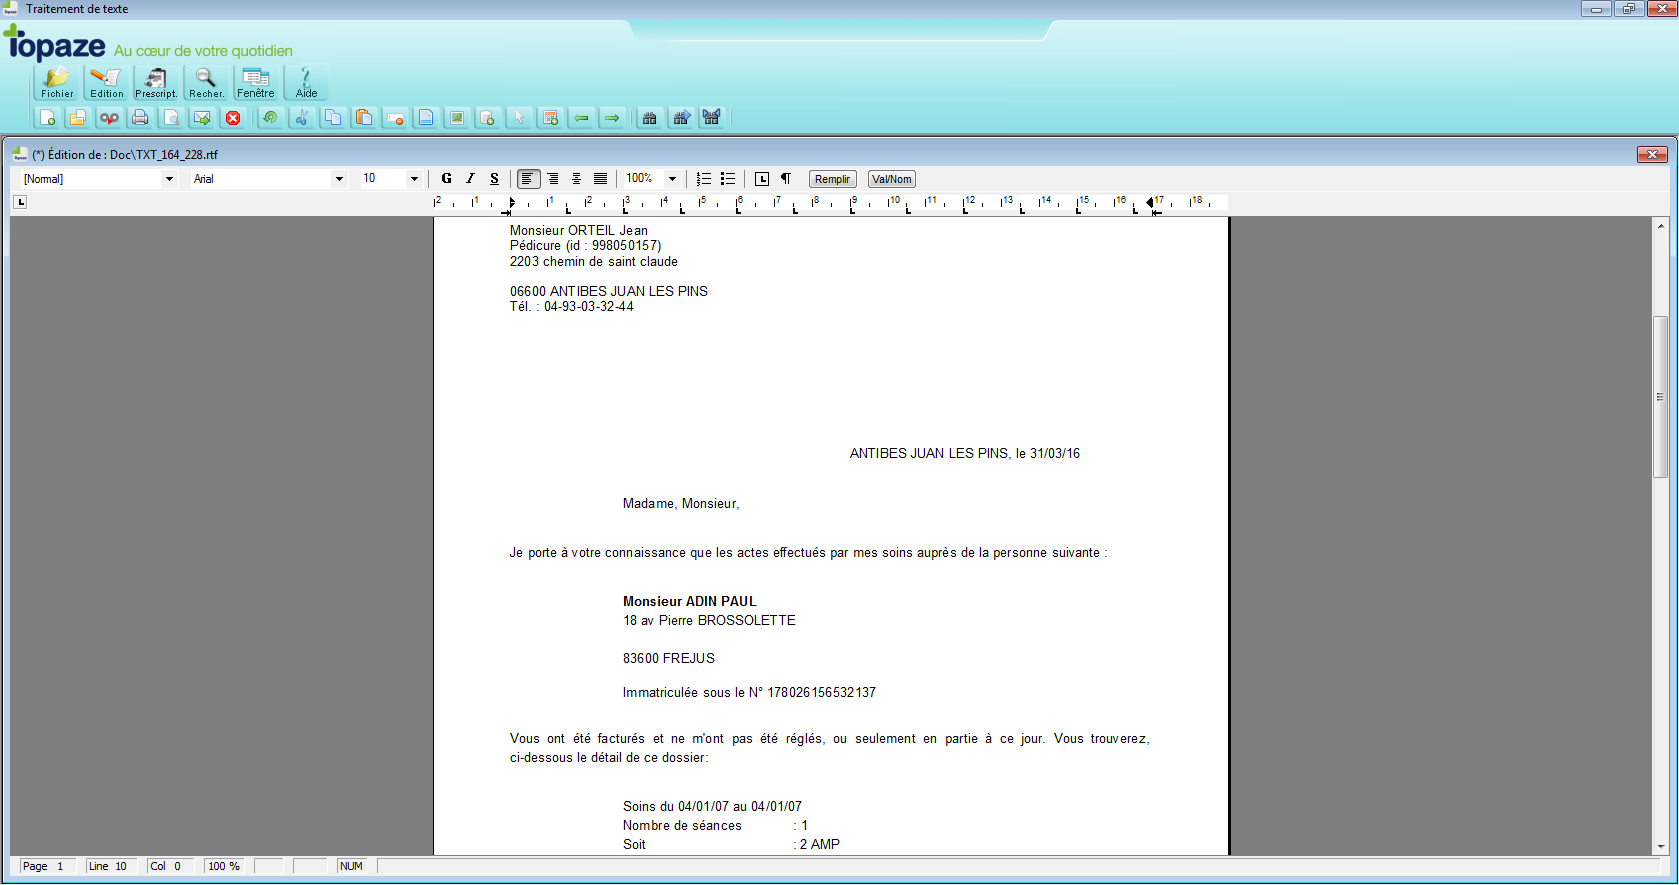
\includegraphics[width=18cm]{./img/text_editor2}
  \caption{\label{fig:editeur_texte} L'éditeur de texte présent dans Topaze Maestro.}
\end{figure}


\newpage
\begin{figure}[H]
\section*{Exemple de modèle XML utilisé par le générateur de code}
  \centering
  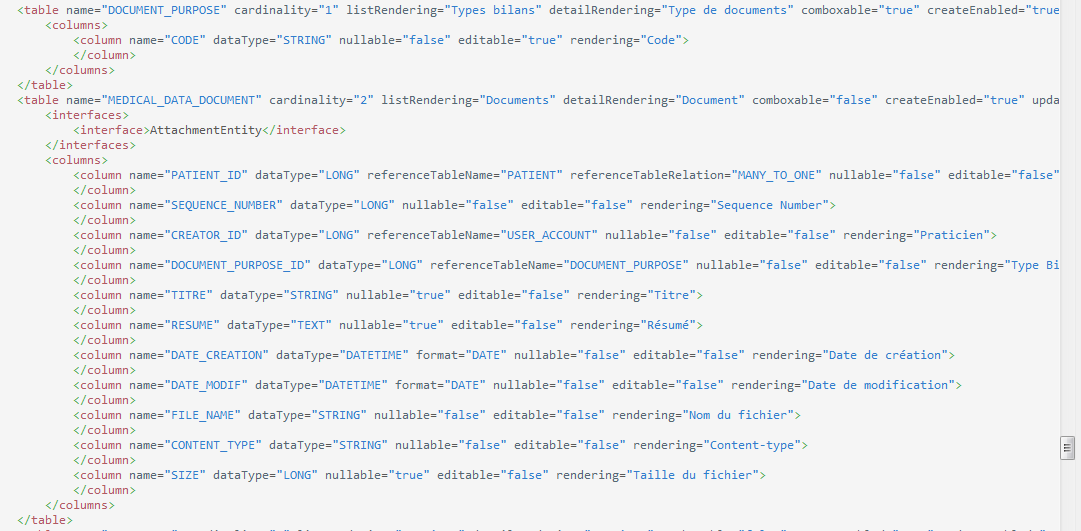
\includegraphics[width=18cm]{./img/modele_generateur}
  \caption{\label{fig:xml} Exemple de modèle décrit en XML à destination du générateur.}
\end{figure}

\begin{figure}[H]
\section*{Diagramme de séquence de la requête d'obtention du dossier médical}
  \centering
  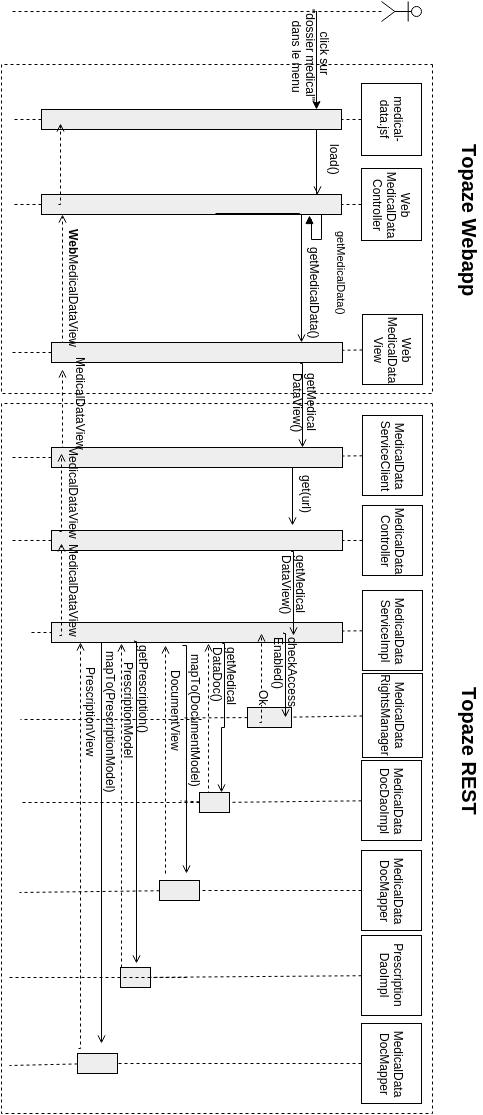
\includegraphics[height=22cm]{./img/diag_seq2}
  \caption{\label{fig:diag_seq} Diagramme de séquence modélisant la requête du dossier médical.}
\end{figure}

\newpage
\begin{figure}[H]
\section*{Le dossier médical de Topaze Web}
  \centering
  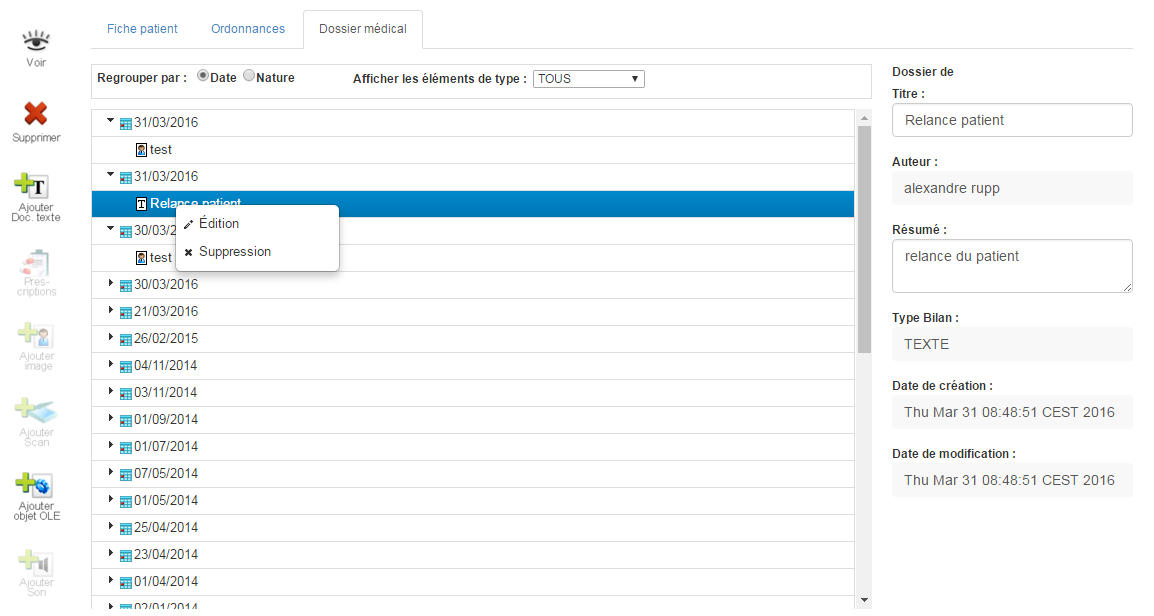
\includegraphics[width=18cm]{./img/dossier_medical_web2}
  \caption{\label{fig:dossier_web} Le dossier médical implémenté dans Topaze Web.}
\end{figure}

\newpage
\begin{figure}[H]
\section*{L'editeur de texte de Topaze Web}
  \centering
  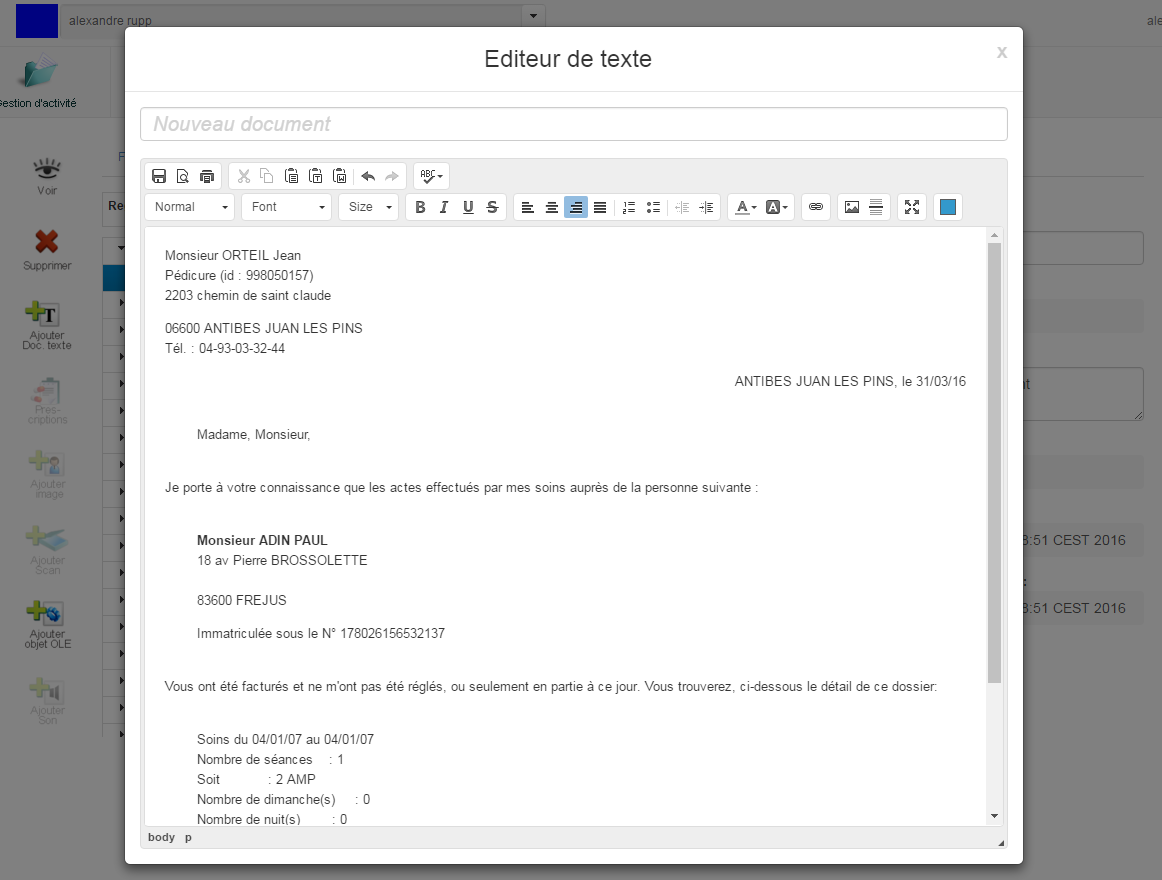
\includegraphics[width=18cm]{./img/editeur_topaze_web}
  \caption{\label{fig:editeur_web} L'éditeur de texte (CKEditor) intégré dans Topaze Web .}
\end{figure}

%\newpage
%\begin{figure}[H]
%\section*{Exemple de classe annotée}
%  \centering
%  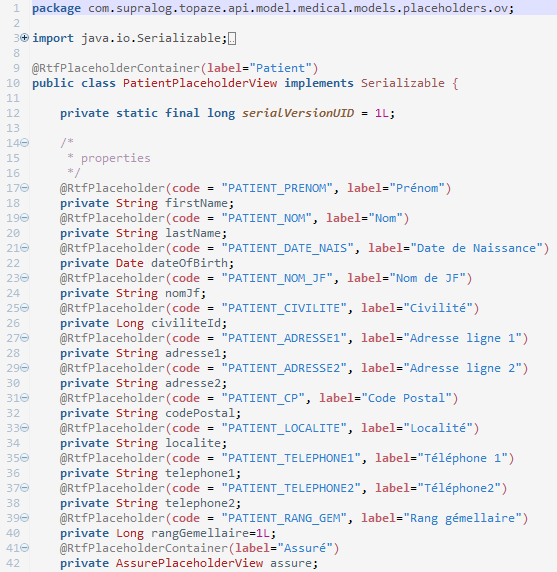
\includegraphics[width=15cm]{./img/annotations}
%  \caption{\label{fig:annotations} La classe Patient a été annotée avec 2 annotations (RtfPlaceholderContainer et RtfPlaceholder) afin de pouvoir être ensuite introspectée et servir à créer l'arborescence de placeholders.}
%\end{figure}

\end{appendices}

